\documentclass[12pt,oneside,a4paper]{article}   
\usepackage[czech, english]{babel}
\usepackage{amsmath}
%\usepackage{epsf,epic,eepic,eepicemu,url,graphicx}
\usepackage{epsf,url,graphicx}
\usepackage[utf8]{inputenc}
\usepackage{float}

%% code listings, pretty simple, but works quite ok :-)
\newenvironment{listing}
{\begin{list}{}{\setlength{\leftmargin}{1em}}\item\scriptsize\bfseries}
{\end{list}}

\begin{document}
\begin{center}
\bf MI-VMW\\[2mm]
    \begin{Large}Flickr - reranking založený na metadatech\end{Large}\\[3mm]
       Michal Sláma (slamamic@fit.cvut.cz)\\
       Šimon Steklík (steklsim@fit.cvut.cz)\\
leden 2016
\end{center}

\section{Zadání}
Cílem projektu je vytvoření aplikace umožňující vylepšené vyhledávání ve fotografiích uložených na serveru
Flickr. Flickr poskytuje aplikační rozhraní umožňující získat prakticky libovolná data o fotografiích, která jsou
přístupna i z oficiálního webového rozhraní. Cílem projektu je tedy aplikace, která umožní vyhledávání na
flickru založené na klíčových slovech, stejně jako je tomu na Flickru nyní, ale navíc bude možné zadat
sekundární vyhledávání na libovolná metadata.

\subsection{Vstupy}
Klíčové slovo, sada hodnot metadat pro setřídění a počet výsledků (omezení velikosti výstupu).
Jako metadata určená k rerankingu jsme zvolili tato:
\begin{itemize}
	\item Řetězec - popis obrázku.
	\item GPS - místo kde byla fotka pořízena.
	\item Integer - počet zhlédnutí obrázku.
	\item Datum - datum pořízení obrázku.
\end{itemize}
U každého z metadat bude možné zvolit jeho váhu (míru důležitosti).

\subsection{Výstup}
Fotky, jejichž popis odpovídá klíčovému slovu. Fotky budou setříděné podle vzdálenosti ke zvoleným
metadatům.

\section{Způsob řešení}
V této sekci je popsán použitý způsob rerankingu obecně a pro jednotlivé typy metadat.

\subsection{Obecné principy}
Reranking se dá obecně popsat jako "znovuseřazení" nějaké už řazené množiny -- v našem případě je první fází vyhledání fotek na Flickeru podle klíčového slova a množina výsledků tohoto hledání je poté seřazena podle "vzdálenosti" k použitým metadatům. Tato vzdálenost se pro různé typy dat počítá rozdílně a existuje mnoho způsobů jejího výpočtu; ve druhé části této kapitoly budou popsány námi vybrané typy výpočtu pro jednotlivé typy metadat.

Tyto vzdálenosti je pak třeba zkombinovat do jedné hodnoty, podle které jsou pak obrázky seřazeny -- toto bude popsáno na konci kapitoly.

\subsection{Typy metadat}
\subsubsection{Řetězec}
Pro výpočet vzdálenosti mezi řetězci jsme zvolili \textit{Levenstheinovu vzdálenost}, která definuje vzdálenost jako počet přidání, odebrání a nahrazení písmen potřebných pro transformaci jednoho řetězce na druhý \cite{Levensthein}.
Např. řetězce \texttt{"rank"} a \texttt{"tank"} mají vzdálenost 1 (výměna "r" za "t"), \texttt{"rank"} a \texttt{"rerank"} jsou ve vzdálenosti 2.

Při implementaci je využito dynamického programování, protože naivní rekurzivní algoritmus si v rozumném čase neporadí s řetězci delšími než cca 10 znaků \cite{Levensthein_java}.

\subsubsection{GPS}
Při výpočtu vzdálenosti mezi dvěma body na zeměkouli (bod kde byla fotografie pořízena a bod vybraný uživatelem) jsme použili \textit{Great-circle Distance}, která počítá vzdálenost dvou bodů na povrchu (ideální) koule \cite{GCD}. Není tedy na Zemi úplně přesná, ale pro naše účely plně postačuje.

\subsubsection{Datum}
Vzdálenost mezi daty (datum pořízení fotografie a datum vybrané uživatelem) počítáme jednoduše jako absolutní hodnotu jejich rozdílu ve dnech.

\subsubsection{Celá čísla}
Vzdálenost mezi celými čísly (počet zklédnutí fotografie a číslo určené uživatelem) počítáme jednoduše jako absolutní hodnotu jejich rozdílu.

\subsection{Kombinace vzdáleností (normalizace, decay funkce)}
Rozsah hodnot jednotlivých typů metadat není stejný (u některých teoreticky neomezený). Mohlo by se tedy stát, že fotografie, která se shoduje ve všech metadatech kromě jednoho, kde je rozdíl hodnot naopak obrovský, bude nesprávně upozaděna oproti fotografii, která se liší ve všech metadatech, ale v řádově menší míře. Je proto třeba vzdálenosti nějakým způsobem \textit{normalizovat} -- převést do určitého společného rozsahu hodnot.

My pro převedení do rozsahu \textit{(0, 1)} používáme tuto \textit{decay funkci}:
\begin{equation}
	f(x) = 1 - e^{-\lambda x}
\end{equation}
kde \(x\) je vypočtená vzdálenost a \(\lambda\) je parametr určující rychlost růstu funkce (čím větší je \(\lambda\), tím rychleji hodnota funkce roste k jedničce). Pro každý typ metadat je \(\lambda\) nastavena jinak (podle předpokládaného rozsahu hodnot daných metadat).

Celkový \textit{rank} (menší je lepší) každé fotografie je pak dán součtem hodnot u všech typů metadat.

\subsection{Váhy metadat}
Uživatel má možnost u každého typu metadat určit, jakou váhu mu přisuzuje -- výsledky s nízkou vzdáleností u daného typu budou pak upřednostněny více nebo méně. Pro naše účely jsme zvolili jednoduchou volbu z 5 hodnot (vah): 0, 0.5, 1, 1.5, 2 (0 ve výsledku vypne řazení podle daného typu metadat).

\section{Implementace}

\subsection{Java}

Aplikace je implementována v programovacích jazyce Java s využitím frameworku Spring s architekturou MVC (Model-View-Controller).
Front-end je pak realizován pomocí jsp a využívá css a javascript od boostrapu a jquery.

Vypíchnout můžeme způsob stažení a rerankingu fotek z flickru. Stažení a reranking je realizováno v samostatných vláknech na principu producent/ konzument. Fotky jsou z flickru staženy vždy po stránkách jejichž velikost je konfigurovatelná pomocí property souboru. Stažené fotky jsou umístěny do sdíleného uložiště mezi oběma vlákny. Reranking průběžně reaguje na stažení nových fotek a pro každou fotku zakládá nové vláknu odpovídající za výpočet rankingu. Vysledekem celého zpracování je list seřazených fotek podle nového rankingu.

\subsection{Knihovny}

Z nejdůležitějších knihoven uveďme (další viz POM projektu):
\begin{itemize}
	\item Spring ve verzi 4.1.1
	\item flickr4java ve verzi 2.13
	\item javax.servlet ve verzi 1.2
	\item slf4j a logback ve verzi 1.75 respektive 1.0.13
\end{itemize}

\subsection{Flicker API}

Pro konzumaci Flicker API je použita knihovna flickr4java. Knihovna odstiňuje od samotné komunikace s Flickerem a poskytuje API s parametrizovaných vstupem a výstupy do objektů odpovídajících specifikaci Flickr API. 

Příklad volání flickr API před knihovnu flickr4java:
\begin{verbatim}
flickr.getPhotosInterface().search(searchParameters, pageLimit, pageOrder);
\end{verbatim}


Applikační beany
\begin{verbatim}
  <bean id="flickrRest" class="com.flickr4java.flickr.REST"/>
  
  <bean id="flickr" class="com.flickr4java.flickr.Flickr">
  <constructor-arg name="apiKey" value="${cz.vmw.flickr.api.apikey}"/>
  <constructor-arg name="sharedSecret" value="${cz.vmw.flickr.api.sharekey}"/>
  <constructor-arg name="transport" ref="flickrRest"/>
  </bean>
\end{verbatim}  
Objekt flickr je vytvořen v kontextu aplikace a konfigurován z property souboru. Nad instancí je možné zvolit potřebné flickr rozhraní. V našem případě definujeme rozhraní pro stažení fotek. Dále už stačí zvolit akci search a dodat potřebné parametry. SearchParameter obsahuje filtr fotek které hledáme (keyword) a specifikuje atributy, které se mají vrátit nad rámek běžné odpovědi (geo, views, description, date\_taken). PageLimit a pageOrder umožňují rozdělit stahování na více oddělených dotazů tak, aby každý stáhl unikátní sadu fotek. Toho v aplikaci využíváme viz. část implementace.
 

\subsection{Požadavky na běh}

Současná verze aplikace byla vyvíjena a nasazena na Glassfish verze 4.1.1 pod Javou 1.7.80. Nejsou použity žádné speciální funkce Glassfish serveru a nic tedy nebrání nasazení do jiných kontejnerů (např. Tomcat, Weblogic, WildFly). U Javy je třeba použít verzi 1.7 a vyšší.

Aplikace potřebuje přístup k internetu, přesněji prostup na API flickru. Další externí požadavky nemá. Díky své jednoduchosti nemá aplikace speciální nároky na systémové zdroje.


\section{Příklad výstupu}
Základní rozvržení aplikace je vidět na obrázku \ref{fig:layout}. Vlevo je vyhledávací formulář, kde je možné nahoře zvolit počet porovnávaných obrázků a klíčové slovo pro hledání na Flickru. Ve spodní části formuláře je pak možné volit hodnoty a váhy (pomocí posuvníků) jednotlivých typů metadat.

Vpravo se pak nachází výsledky vyhledávání - karty obrázků, které obsahují celkové skóre obrázku a hodnoty jednotlivých metadat. Po kliknutí na náhled obrázku se stánhe a zobrazí jeho větší verze.

\begin{figure}[H] \begin{center}
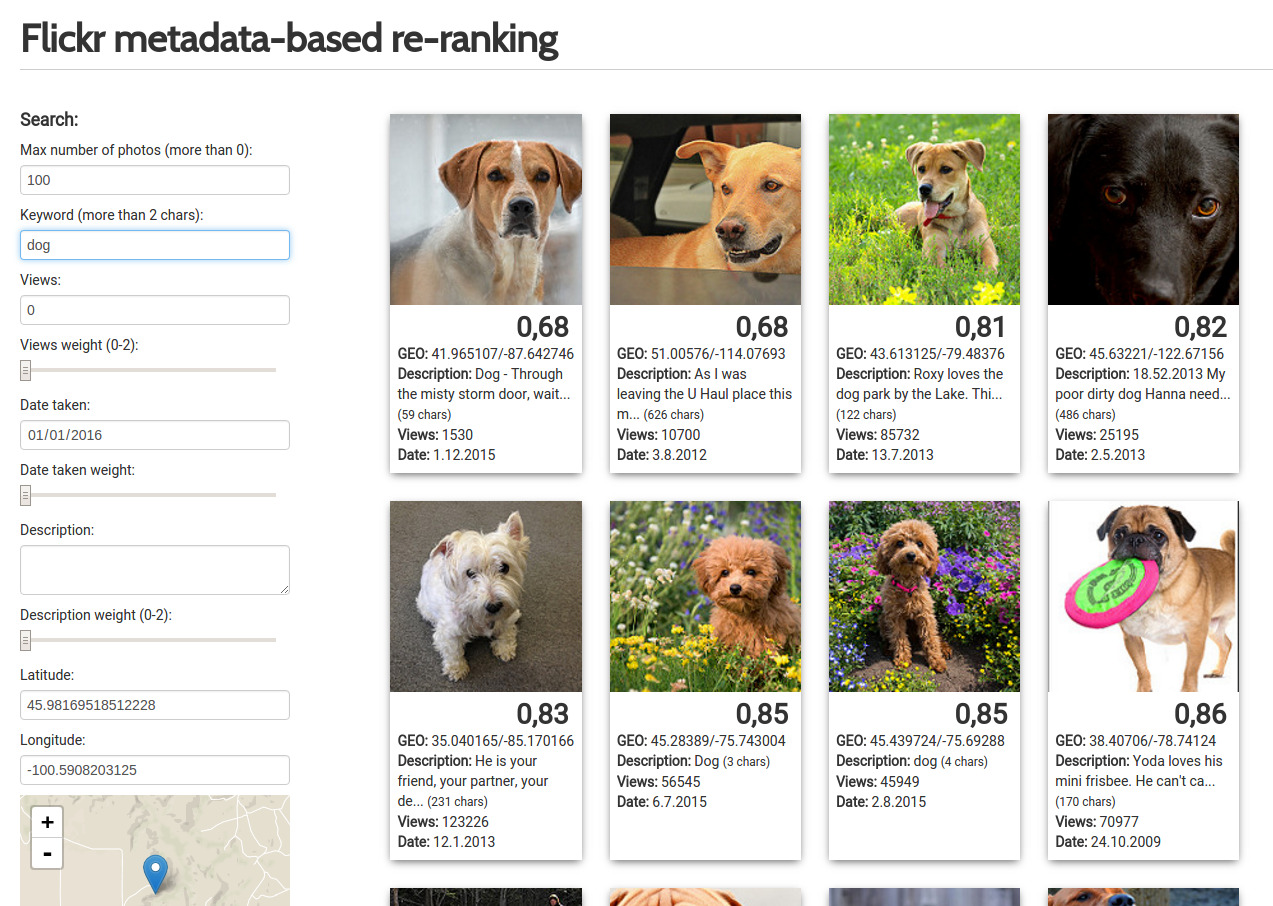
\includegraphics[width=13cm]{pics/layout.png} \caption{Rozvržení aplikace}
\label{fig:layout}
\end{center} \end{figure}

\subsection{Vyhledávání bez/s re-rankingem}
Jako příklad uvádíme vyhledání klíčového slova \texttt{"dakota"}, s tím, že uživatele zajímají fotky ze (Severní/Jižní) Dakoty v USA. Při prostém vyhledávání bez re-rankingu (stahujeme 100 fotek) se sice zobrazí i fotografie z Dakoty, ale jak je vidět na obrázku \ref{fig:dakota_no_geo} kromě nich také fotografie herečky Dakoty Fanning, letadla Douglas DC-3 Dakota a další. Ve výsledku jsou fotografie, které hledáme, v menšině.



\begin{figure}[H] \begin{center}
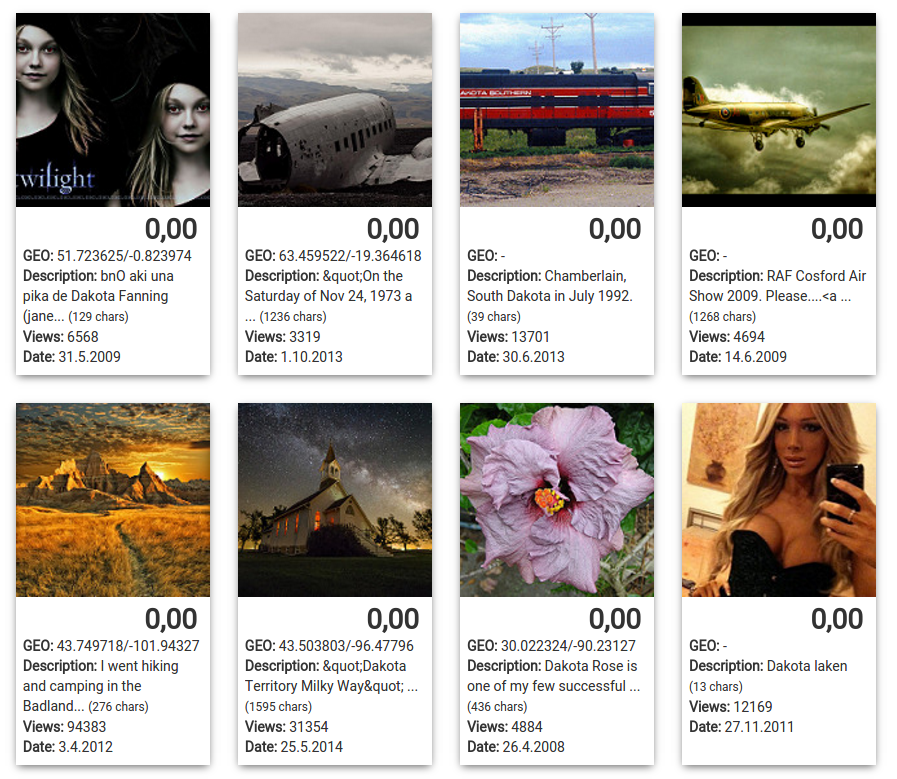
\includegraphics[width=13.5cm]{pics/dakota_no_geo.png} \caption{Vyhledání slova "dakota" bez re-rankingu (prvních 8 výsledků)}
\label{fig:dakota_no_geo}
\end{center} \end{figure}

Při určení požadované polohy fotky (někde na rozmezí Severní a Jižní Dakoty) jsou výsledky diametrálně odlišné -- většina fotografií na prvních pozicích ukazuje přírodu v Dakotě a jinak tematicky zaměřené fotky jsou daleko vzadu (obrázek \ref{fig:dakota_geo}).

\begin{figure} \begin{center}
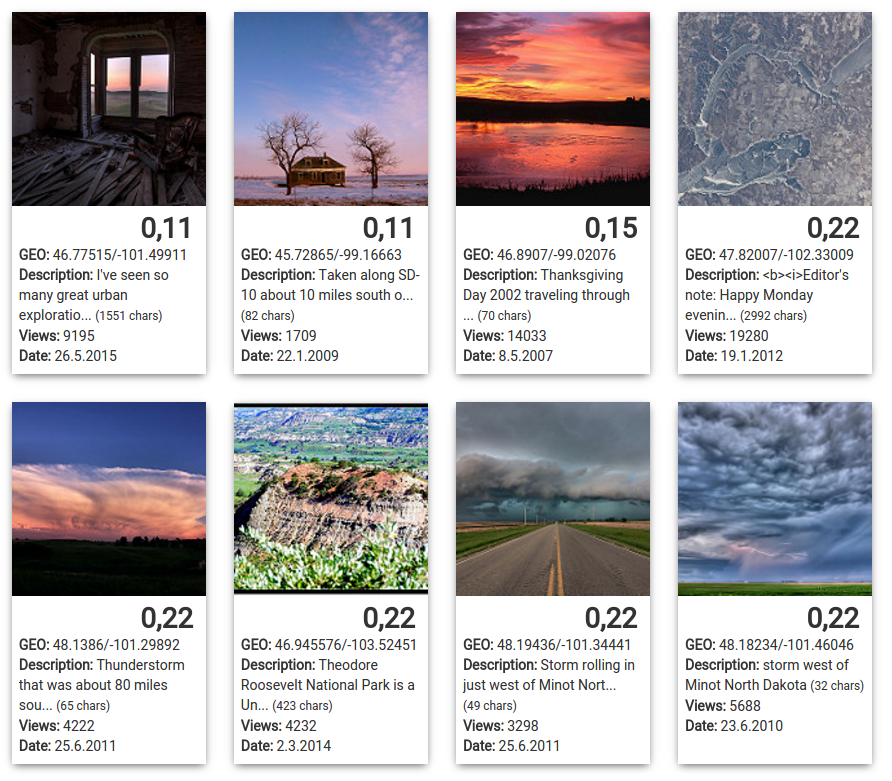
\includegraphics[width=13.5cm]{pics/dakota_geo.png} \caption{Vyhledání slova "dakota" s re-rankingem (prvních 8 výsledků)}
\label{fig:dakota_geo}
\end{center} \end{figure}


\section{Experimentální sekce}
- ze zadání: "Většina projektů lze posuzovat z hlediska přesnosti či rychlosti (nebo obojího),
přičemž tyto jsou závislé na různých vstupních parametrech projektu. V této sekci by
měly být takové parametry zkoumány. Např. rychlost typicky závisí na velikosti
vstupu nebo naopak velikosti výstupu. Lze pak například do grafu nebo tabulku
vynést takovéto závislosti."

\section{Diskuze}
\iffalse
- zadání: "Většina projektů je typu “proof of koncept“, tj. jde o vyzkoušení poznatků
prezentovaných v přednáškách v praxi. Nejde tedy o detailní řešení všech problémů,
které mohou při implementaci nastat – takový projekt by dalece přesahoval rámec
semestrálního projektu. Tato sekce tedy obsahuje rozbor těchto nedostatků a
potenciálním způsobu jejich řešení."
\fi
V projektu zkoušíme řazení podle čtyř typů metadat -- poloha, datum, celé číslo, řetězec. Bylo by samozřejmě možné provádět re-ranking i podle dalších atributů fotografií (např. podle jejich velikosti, poměru stran, \ldots), nicméně principy jsou obdobné. Mohli bychom také např. zohledňovat, v jakém pořadí vrací Flickr fotografie v základním dotazu pomocí klíčového slova.

Naše aplikace také řadí velmi malou podmnožinu fotografií na Flickru -- vždy v reálném čase stáhne daný počet fotografií a porovnává pouze je. Tento nedostatek by se dal vyřešit indexací (části) databáze Flickru do lokální databáze a prací nad těmito daty. Nicméně samotný algoritmus porovnávání by nebylo třeba nijak upravovat -- je nezávislý na množství a zdroji dat.



\section{Závěr}
V rámci semestrální práce jsme se seznámili s principy re-rankingu a navrhli a implementovali webovou aplikaci provádějící re-ranking fotografií ze služby Flickr na základě jejich metadat. V rámci práce na aplikaci jsme naučili využívat některé algoritmy na měření vzdáleností mezi numerickými i nenumerickými hodnotami, např. Levenstheinovu (editační) vzdálenost pro měření vzálenosti mezi dvěma řetězci. Dále jsme si vyzkoušeli, jak dané vzdálenosti kombinovat a normalizovat.

- něco k implementaci? Napsat ja parádně naše aplikace funguje?

\iffalse
v============== cizí semestrálka ================v

\section{Použité technologie}

%Rozhodli jsme se použít programovací jazyk Java. Protože nedílnou součástí naší práce je i~webové rozhraní, použijeme variantu Java Enterprise Edition (Java EE). Jako aplikační platformu jsme vybrali volně dostupný, veřejně přístupný a~snadno škálovatelný systém Google App Engine \cite{GoogleAE}, který zdarma poskytuje serverový prostor pro aplikace naprogramované i~v~Java EE.

Pro vývoj jsme použili verzovací systém git, konkrétně veřejně přístupný portál github.com \cite{official}. Pokud je v textu odkazováno k~nějaké vývojové větvi, naleznete ji právě tam.

\section{Získávání obrázků ze serveru Flickr}
Vzhledem k volbě programovacího jazyka bylo pro přístup k API služby Flickr nejjednodušším řešením využití existující knihovny flickrj \cite{flickrj}. Práce s~ní je přitom velice jednoduchá, jak ukazuje následující příklad.

\begin{listing}
\begin{verbatim}
Flickr flickr = new Flickr(API_KEY, SHARED_SECRET, new REST());
SearchParameters sp = new SearchParameters();
sp.setText(keyword);
PhotoList result = flickr.getPhotosInterface().search(sp, perPage, page);
\end{verbatim}
\end{listing}

Výsledkem této sekvence kódu je seznam objektů vyhovujících zadaným parametrům a nacházejících se na dané straně při určeném počtu výsledků na jedné straně.

Tyto objekty v~sobě nesou bližší informace o konkrétní fotografii, kterou reprezentují. Jsou jimi např. identifikátor, rozměry, URL náhledů v~různých velikostech, atd. Objekt taktéž obsahuje metody, které umožňují získat fotografii k~dalšímu zpracování rovnou v~podobě objektu BufferedImage.

V této souvislosti práce rovněž implementuje jednoduchou cache, která uchovává posledních 50 výsledků hledání, čímž výrazně zrychluje její chod při opakování dotazu se stejným klíčovým slovem.

\section{Hodnocení obrázků}
Pro hodnocení a~řazení obrázků podle referenční barvy se nabízí relativně mnoho postupů a~algoritmů, my jsme se v~naší práci rozhodli zaměřit na rychlost a~zpracování výsledků pokud možno v~reálném čase. Běžnou praxí podobných vyhledávačů je totiž stažení nějakého většího vzorku obrázků, jejich off-line ohodnocení a~posléze uživateli nabízí jen vyhledávání v~této omezené databázi.

Naše implementace se naopak snaží uživateli nabídnout vždy ty poslední fotografie k~daným klíčovým slovům, ačkoliv se některé vypočítané hodnoty ukládají do databáze tak, aby časově náročné výpočty probíhaly pokud možno pro každou fotografii jen jednou.

\subsection{Možnosti porovnávání}
První možností, která se nabízí pro srovnávání barevnosti obrázků s~referenční barvou je metoda popsaná v~\cite{Mueller2k9}. Ta je založená na vytvoření omezené palety barev, na něž se mapuje barva jednotlivých pixelů v~obrázku. Po analýze pixelů tak vznikne histogram této omezené palety, pomocí něhož se dá spočítat vzdálenost různých obrázků vůči referenční barvě, která je rovněž namapována do základní omezené palety barev. Tato metoda se vyznačuje tím, že se výsledná sada obrázků dá velice snadno dále třídit podle dalších barev.

Druhou variantou, která okamžitě vytane na mysl je porovnávání obrázků založené na klasickém RGB histogramu. Jakmile máme spočítaný histogram obrázku, můžeme volit různé metriky pro počítání vzdálenosti od referenční barvy.

\subsection{Extrahované vlastnosti}

V~průběhu implementace jsme zkoušeli subjektivně porovnávat obě metody, a~přišlo nám, že na omezenou sadu obrázků, kterou jsme schopni zpracovat v~pseudo-reálném čase fungují o~něco lépe metody založené na porovnávání RGB histogramů. Co se týče výpočetní a~časové náročnosti, jsou obě metody v~podstatě srovnatelné. Implementace algoritmu vycházejícího z~\cite{Mueller2k9} je dostupná v~repozitáři \cite{official} ve vývojové větvi \textbf{piximilarlike}.

V naší finální implementaci používáme druhou metodu založenou na kompletních RGB histogramech. Po získání výsledků vyhledávání ze serveru Flickr tak dochází k~výpočtu histogramu pro každý obrázek pro všechny tři kanály barevného prostoru RGB. Takto získaný histogram je uložen do databáze, kde se uchovává pro budoucí výpočty se stejným obrázkem.

\subsection{Podobnost k referenční barvě}
\label{sec:podobnost}

Pro modelování podobnosti jsme zkoušeli několik metod s~různými úpravami, vždy jsme se však museli držet relativně nízké výpočetní náročnosti kvůli omezení na zpracování v~pseudo-reálném čase.

Nejprve jsme zkoušeli obrázky řadit podle vážené euklidovské vzdálenosti mezi referenční barvou a~nejčastější barvou nacházející se ve spočítaném histogramu (vývojová větev \textbf{peakdistance}). Výsledky takových porovnání nás však příliš neuspokojily a~snažili jsme se nalézt jiné metody.

Nakonec jsme došli k~metodě, která na první pohled nemusí vypadat zcela dokonale, nicméně pro danou aplikaci podává subjektivně poměrně dobré řešení v~rozumném čase. Charakteristické číslo pro každý obrázek, podle kterého budeme obrázky v~této variantě řadit, budeme označovat jako \textbf{váhu obrázku}.

Váha obrázku se vždy skládá ze součtu tří charakteristických čísel vychá-zejících z~histogramů jednotlivých složek RGB modelu. Tato charakteristická čísla jsou počítána podle následujícího algoritmu, kde \texttt{EPSILON} je předem stanovená konstanta, \texttt{baseIndex} je hodnota příslušného kanálu z~referenční barvy a~\texttt{HIST\_SIZE} je šíře histogramu pevně nastavená na 256.

\begin{listing}
\begin{verbatim}
for (int i = baseIndex - EPSILON; i < baseIndex + EPSILON; i++) {
    if (i >= PhotoHistogram.HIST_SIZE) { break; }
    if (i < 0) { continue; }
    sum += histogram.getValue(color, i) *
        (i - baseIndex == 0 ? 1 : Math.abs(i - baseIndex));
    ++values;
}
return (sum / values == 0.0 ? Double.MAX_VALUE : sum / values);
\end{verbatim}
\end{listing}

Algoritmus projde \texttt{EPSILON} okolí referenční barvy a~postupně nasčítá násobky jednotlivých hodnot v~histogramu. Čím dále se pak hodnota nachází od referenční barvy, tím víckrát se do součtu započítává. V případě, kdy by se v daném intervalu \texttt{baseIndex-EPSILON..baseIndex+EPSILON} nacházely samé nulové hodnoty, je takový součet na závěr nahrazen nekonečnem. To zajišťuje, že obrázky, které nemají žádné body alespoň trochu podobné dané barvě, získávají největší váhu a~propadají se řazeným výsledkem dolů. Pos-lední operací je zprůměrování hodnot tak, abychom nemuseli pracovat s~ob-rovskými čísly. Jako nejpodobnější dané barvě je určen obrázek s~\textbf{nejmenší} vahou.

Algoritmus se dá ladit volením hodnoty konstanty \texttt{EPSILON}. Subjektivně nejlepší výsledky algoritmus podává paradoxně při takové hodnotě, kdy se ve smyčce projde celá šířka histogramu.

Zvolený algoritmus má jistě celou řadu menších či větších nedostatků, například není použita žádná metoda normalizace histogramů. To znamená, že obrázky menších rozměrů mají teoretickou výhodu, protože počet jejich pixelů je nižší. Jelikož však načítáme normované obrázky ze serveru Flickr, můžeme tento faktor zřejmě zanedbat.

Na druhou stranu se nám subjektivně zdá, že pro zvolenou aplikaci běžící takřka v~reálném čase je algoritmus poměrně slušně použitelný, ačkoliv docela často dochází k~jasně zřetelným anomáliím.

\subsection{Komentovaná ukázka řazení obrázků}

\begin{figure} \begin{center}
\includegraphics[width=13.5cm]{figs/histogram1.png} \caption{Histogram prvního obrázku}
\label{fig:manchild}
\end{center} \end{figure}
\begin{figure} \begin{center}
\includegraphics[width=13.5cm]{figs/histogram6.png} \caption{Histogram šestého obrázku}
\label{fig:borderflower}
\end{center} \end{figure}
Pro ilustraci výhod a~nevýhod algoritmu se nyní podívejme na konkrétní příklad řazení.

Celkem řadíme devět obrázků, pro ukázku jsou pro dva konkrétní obrázky uvedeny na obr.~\ref{fig:manchild}~a~ obr.~\ref{fig:borderflower} tři RGB histogramy: normální, ohodnocený pro barvu \verb|#279AF2| a~ohodnocený pro barvu \verb|#362333|. Ohodnoceným histogramem zde rozumíme hodnoty vypočítané pomocí algoritmu uvedeného v~\ref{sec:podobnost}. Šedou čarou je poté vyznačena hodnota kanálu referenční barvy. Pod ohodonocenými histogramy je uvedena i~celková suma těchto hodnot, která vždy slouží jako váha obrázku. Je také nutné čtenáře upozornit, že osy $y$~jednotlivých histogramů mají odlišná měřítka.

\begin{figure} \begin{center}
\includegraphics[width=13.5cm]{figs/col01-flower-279af2-withcolor.png} \caption{Obrázky seřazené podle barvy \#279AF2}
\label{fig:279af2}
\end{center} \end{figure}
\begin{figure} \begin{center}
\includegraphics[width=13.5cm]{figs/col01-flower-362333-withcolor.png} \caption{Obrázky seřazené podle barvy \#362333}
\label{fig:362333}
\end{center} \end{figure}

Jak dopadlo výsledné řazení se můžeme podívat na obrázcích \ref{fig:279af2} a~\ref{fig:362333}, kam jsme pro ilustraci doplnili čtverec vyplněný barvou, podle které řadíme. Na ukázkových obrázcích \ref{fig:manchild} a~\ref{fig:borderflower} si nyní ukážeme, jak reálně funguje náš algoritmus.

Už u~standardního histogramu je vidět veliký rozdíl v~rozmístění bodů na šíři histogramu. U~obr. \ref{fig:borderflower} vidíme velikou špici u černé barvy, kterou způsobuje černý pruh u~horního a~spodního okraje obrázku. Díky tomu, že v~jednom místě je hodnota výrazně vyšší, než v~těch ostatních, bude algoritmus dobře fungovat v~blízkosti tohoto místa, okolí daného bodu bude započítáno s~nejmenším koeficientem a~vzdálenější místa s~nižšími hodnotami nedají v~součinu tak velká čísla. Oproti tomu při rovnoměrném rozvrstvení hodnot histogramu nebude vzdálenost od referenčního bodu hrát příliš velkou roli.

V~prvním řazení podle barvy \verb|#279AF2| je jako podobnější vyhodnocen obrázek \ref{fig:borderflower}. Je to dáno tím, že do výsledného součtu přispívá většinou malými čísly, jediným velkým číslem je vždy špice u~levého kraje histogramu. Fotografie \ref{fig:manchild} doplácí na to, že jediným ze tří histogramů, kde dochází k~výrazné změně rozložení jednotlivých podílů na výsledném součtu je červený kanál.

U~řazení podle barvy \verb|#362333| se situace obrací. Na obr. \ref{fig:manchild} je krásně vidět, jak se v~modrém a~zeleném histogramu dramaticky změnilo rozdělení jednotlivých podílů na celkovém součtu, kdežto u~obrázku \ref{fig:borderflower} se prakticky nic nezměnilo. Tím, že jsme "trefili" skoro nejčastější barvu v~obrázku \ref{fig:manchild} jsme zajistili její nejnižší podíl na celkovém součtu a~tím v~podstatě i~nejnižší možný celkový součet.

V~součtech u~obrázku \ref{fig:borderflower} si můžeme také všimnout vždy obrovského přís-pěvku modrého kanálu. Opět jde o~efekt jedné velké špice, která (skoro) vždy přispěje velkou měrou do celkového součtu.

Velkou nevýhodou algoritmu je nezávislé posuzování tří kanálů barevného prostoru RGB. Při řazení může dojít k~situaci, kdy nás reálně zajimá řazení pouze podle jednoho kanálu (např. barva \verb|#FF0000|), díky tomu, že vahou je součet součtů všech kanálů nám do řazení zasáhnou i~zbylé dva kanály. Teoreticky zvýhodněny tak budou velmi tmavé obrázky, které obsahují hodně hodnot blízkých nule v~kanálech G~a~B. To může vést k~leckdy zavádějícím výsledkům.

\section{Implementační poznámky}

Google App Engine bohužel neumožňuje použití některých standardních knihoven a~tříd jazyka Java, a~proto jsme museli v~některých částech aplikace sáhnout k~náhradním řešením.

%Naše aplikace tak musí obsahovat vlastní implementaci dekodéru formátu JPEG, který jsme převzali z~\cite{Dersch}, protože GAE nepodporuje použití Javovské třídy BufferedImage.

\section{Závěr}

Myslíme si, že v~rámci semestrální práce se nám povedlo implementovat docela použitelný hodnotící algoritmus, který vyniká poměrně velkou rychlostí, jež je bohužel vykoupena nepřesností algoritmu. Použitá váha obrázku není zcela špatná a~po zapojení některých metod na eliminaci například velkých špicí v~histogramech by se její účinnost mohla ještě zlepšit.

%Aplikace je veřejně dostupná na \cite{liveApp}, zdrojové kódy jsou veřejně přístupné k nahlédnutí na \cite{official}.

\fi

\renewcommand{\refname}{Literatura}
\bibliographystyle{ieeetr}
{
 \bibliography{refs}
}
\end{document}